\documentclass[11pt, class=article, crop=false]{standalone}
\usepackage{amsmath,amssymb,amsfonts,amsthm}
\usepackage{enumitem}
\usepackage{fancyhdr}
\usepackage{tikz-cd}
\usepackage{mathabx}
\usepackage{geometry}
\usepackage{natbib}
\usepackage{braket}
\usepackage{graphicx}
\usepackage{simpler-wick}
\usepackage{hyperref}
\usepackage{cancel}
\usepackage{listings}
\usepackage{relsize}
\usepackage{xcolor}
\usepackage{stmaryrd}
\usepackage{tikz-feynman}
\usepackage{kiritsis}
\geometry{margin = 0.5in}


\begin{document}
\section*{Chapter 6: Strings in Background Fields} % (fold)
\label{sec:chapter_6_strings_in_background_fields}
Note this chapter is specific to \emph{closed oriented strings}. As such, we will not consider the effects of the boundary.
\begin{enumerate}
	\setcounter{enumi}{-1}
	\item This is not a required problem but it certainly should be \footnote{After seeing the details of this calculation, I can understand why it was omitted.}. Let's \emph{calculate the $\beta$-functions of the nonlinear sigma model}. Here, I will borrow diagrams from the very nice set of TASI lecture notes of Callan and Thorlacius 
	
	First, it is worth using a normal coordinate system for the $X^\mu$ (one in which all of the $\Gamma$ symbols vanish and all higher symmetrized $\Gamma$ symbols also vanish). % Then, in a normal coordinate system we can write:
 	% \[
 	% 	T(X_0 + \eta) = \sum_{m=0}^\infty \frac{1}{m!} \d_{\nu_1} \dots \d_{\nu_m} T(X_0) \eta^{\nu_1} \dots \eta^{\nu_m}
 	% \]
	We want to look at radiative corrections to $\braket{T_{++}}$, since they have integrals that are easier to handle than those for $\braket{T_{+-}}$. From conservation this will give us the trace anomaly for $\braket{T_{+-}}$. We will first look at how $G$, $B$ affect the trace on a flat worldsheet.
	
	For the graviton contribution to $\beta^G$, we have only only one diagram
	\begin{center}
		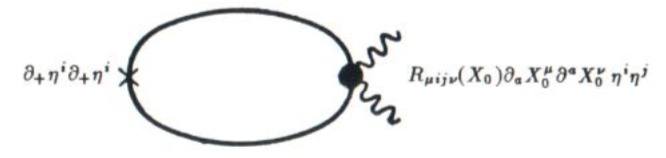
\includegraphics[scale=0.6]{Figures/G}
	\end{center}
	This contributes an anomalous trace of
	\[
		\braket{T_{+-}} = \frac14 R_{\mu \nu} \, \partial_a X^\mu_0 \partial^a X^\nu_0
	\]
	
	For the $B$ contribution to $\beta^B$, we have two such diagrams:
	\begin{center}
		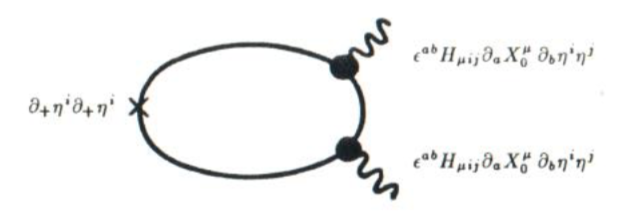
\includegraphics[scale=0.6]{Figures/B1} \quad 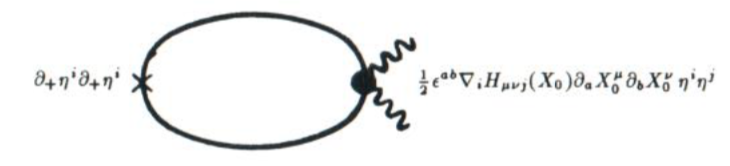
\includegraphics[scale=0.6]{Figures/B2}
	\end{center}
	These contribute anomalous traces of:
	\[
		-\frac{1}{16} H_{\mu \rho \sigma} H_{\nu \rho \sigma} \,  \partial_a X^\mu_0 \partial^a X^\nu_0, \quad \frac18 \nabla^\lambda H_{\mu \nu \lambda} \epsilon^{ab}  \partial_a X^\mu_0 \partial_b X^\nu_0
	\]
	respectively.
	
	The dilaton contribution \emph{also} affects the trace on the flat world sheet (even though it does not couple at $R=0$), by affecting the stress energy tensor as it is defined by varying the action w.r.t. the metric. Kiritsis has worked this out before and shown that the dilaton contributes $(\d_a \d_b - g_{ab} \Box) \Phi$ to the stress energy tensor, from which we get a dilaton contribution of $\Box_\xi \Phi(X(\xi))$ to the trace. Using covariant expressions for the D'alambertian we arrive at a contribution
	\[
		\nabla_\mu \nabla_\nu \Phi(X_0) \, \d_a X_0^\mu \d^a X_0^\nu - \frac12 \nabla^\lambda \Phi(X_0) H_{\mu \nu \lambda} (X_0) \d_a X_0 \d_b X_0 \epsilon^{ab}
	\]
	Combining all of this together, we see that we will get the $\beta$-functions:
	\[
		\beta^G = R_{\mu \nu} - \frac14 H_{\mu \rho \sigma} H_{\nu}^{\rho \sigma} + 4 \nabla_\mu \nabla_\nu \Phi, \quad \beta^B = - \frac12 \nabla^\lambda H_{\lambda \mu \nu} - 2 \nabla^\lambda \Phi H_{\lambda \mu \nu}.
	\]
	As pointed out, these are not quite that RG beta functions (for example compare $\beta^B$ to the correct form in Kiritsis), but around the fixed point, they capture the correct first order behavior. In particular their vanishing will mean that we have no Weyl anomaly. 
	
	Now we need to account for the effects of a curved worldsheet geometry. We can account for this by looking at a $\braket{T_{+ -} T_{+ -}}$ correlator:
	\begin{equation}\label{eq:vartrace}
		\frac{\delta}{\delta \phi(\xi)} \braket{T_{+-} (0)}_{e^\phi \delta_{ab}} = -\frac{1}{4\pi} \braket{T_{+ -}(\xi) T_{+ -}(0)}_{\delta_{ab}}
	\end{equation}
	 Again we can get this by first looking at $\braket{T_{++} T_{++}}$ and appealing to conservation. The Weyl anomaly comes from this diagram:
	\begin{center}
		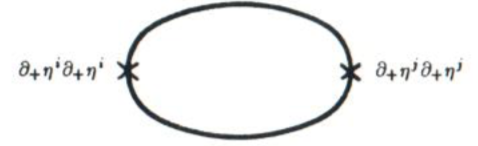
\includegraphics[scale=0.6]{Figures/Phi0}
	\end{center}
	This gives $\braket{T_{+-} T_{+-}} = \frac{\pi D}{12} \Box \delta^{(2)}(\xi)$. Here we have a factor of $D$ coming from each degree of freedom. This can be used to integrate equation \eqref{eq:vartrace} to yield:
	\[
		\braket{T_{+-}} = -\frac{D}{48} \Box \phi = \frac{D}{24} \sqrt \gamma\, R
	\]
	Note that the ghosts (which are otherwise decoupled) will here contribute their factor of $-26$.
	
	We also now need to consider \emph{two-loop} contributions of $G, B$ to the $TT$ correlator. The following diagrams contribute:
	\begin{center}
		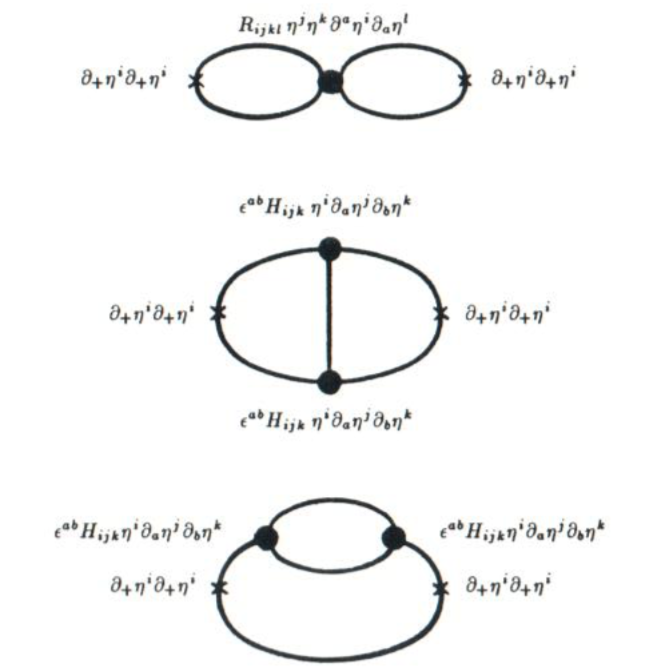
\includegraphics[scale=0.6]{Figures/Phi1}
	\end{center}
	The calculations here are very involved, but will precisely give us
	\[
		\frac{\alpha}{8} (-R + \frac{H^2}{12})
	\]
	Finally, the dilaton both modifies the energy-momentum tensor, giving rise to a tree-level propagator contribution to the two-point function:
	\begin{center}
		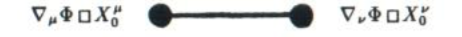
\includegraphics[scale=0.6]{Figures/Phi2}
	\end{center}
	This contributes $\braket{T_{+-}^{dil} T_{+-}^{dil}} = \pi \alpha' (\nabla \Phi)^2 \Box \delta^{(2)}(\xi)$ which will integrate to give a factor of $\frac{\alpha'}{2} (\nabla \Phi)^2\, \sqrt\gamma R$. 
	
	Also, the dilaton gives a loop-contribution to the unmodified energy-momentum tensor:
	\begin{center}
		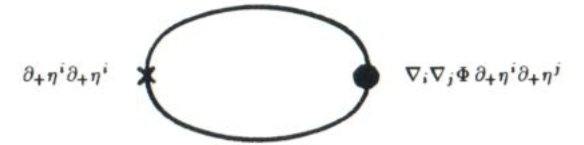
\includegraphics[scale=0.6]{Figures/Phi3}
	\end{center}
	Which contributes the term $\braket{T_{+-}^{dil} T_{+-}^{dil}} = -\pi \alpha' \Box \Phi \Box \delta^{(2)}(\xi)$ which will integrate to give a factor of $-\frac{\alpha'}{2} \Box \Phi \sqrt\gamma R$.
	
	Altogether this gives:
	\[
		\beta^\Phi = D - 26 + \frac32 \alpha' \left[4 (\nabla \Phi)^2 - 4 \Box \Phi - R + \frac{1}{12} H^2 \right].
	\]
	as required. 
	
	\item Each $\beta$-function of a coupling constant $G, B, \Phi$ as given in \textbf{6.1.5, 6.1.6, 6.1.7} is $\frac{\delta}{\delta \phi}$ of that coupling constant, since our scaling $\mu = e^{\phi} \Rightarrow \log \mu = \phi$. Since 
	\[
		T^{a}_{a} = \frac{\beta^\Phi}{12} R^{(2)} + \frac{1}{2 \ell_s^2} (\beta_{\mu \nu}^G g^{\alpha \beta} + \beta^{B}_{\mu \nu} \varepsilon^{\alpha \beta}) \d_\alpha X \d_\beta X
	\]
	The change in effective action under an infinitesimal Weyl transformation $\delta g^{\alpha \beta} = - g^{\alpha \beta} \delta \phi$ is
	\[
		\delta \log Z = - \delta S = \frac{1}{4\pi} \int d^2 \xi \sqrt g T^a_a \delta \phi = \frac{1}{4\pi} \int d^2 \xi \left[ \frac{\beta^\Phi}{12}\,  \sqrt g R^{(2)} + \frac{1}{2 \ell_s^2} \left(\beta_{\mu \nu}^G  \sqrt g\, g^{a b} + \beta^{B}_{\mu \nu} \varepsilon^{a b}\right) \d_a X \d_b X \right] \delta \phi
	\]
	We can integrate this to get the change after a finite conformal transformation:
	\[
		\frac{1}{4\pi} \int d^2 \xi \left[\sqrt g \beta^\Phi \left(R^{(2)} \phi - \frac12 g^{ab} \nabla_a \phi \nabla_b \phi \right) + \frac{\phi }{2\ell_s^2} \left(\beta^G_{\mu \nu} + \beta^B_{\mu \nu} \epsilon^{ab} \right) \d_a X \d_b X \right]
	\]
	this vanishes, of course, when all beta functions are zero. When $\beta^G, \beta^B$ are zero we can show (exercise 3) that $\beta^\Phi$ is a constant, and we recover the Liouville action from before. 
	
	\item First write $G$ explicitly in the action:
	\[
		S = \frac{1}{2\kappa^2} \int d^D x \sqrt{- \det G } e^{-2 \Phi} \left[R + 4 G^{\alpha \beta} \nabla_\alpha \Phi \nabla_\beta \Phi - \frac{1}{12} G^{\alpha \delta} G^{\beta \epsilon} G^{\gamma \zeta} H_{\alpha \beta \gamma} H_{\delta \epsilon \zeta} + 2 \frac{26 - D}{3 \ell_s^2} \right]
	\]
	 The classical equations of motion from varying the action with respect to $G$ give
	\begin{equation}\label{eq:Gvar}
	\begin{aligned}
			0 &= \overbrace{R_{\mu \nu} + 2 \nabla_\mu \nabla_\nu \Phi - \cancel{4 \nabla_\mu \Phi \nabla_\nu \Phi}  - 2 G_{\mu \nu} \Box \Phi + 4 G_{\mu \nu} (\nabla \Phi)^2}^{R \text{ variation}} + \overbrace{\cancel{4 \nabla_\mu \Phi \nabla_\nu \Phi}}^{(\nabla \Phi)^2 \text{ variation}}\\
			& \quad \underbrace{-\frac14 H_{\mu \rho \sigma} H_{\nu}^{\rho \sigma}}_{H^2 \text{ variation}}  \underbrace{- \frac12 G_{\mu \nu} \left( R + 4 (\nabla \Phi)^2 - \frac{1}{12} H^2 + \frac{2}{3 \ell_s^2} (26-D)  \right)}_{\sqrt{-\det G} \text{ variation}}\\
			& = \underbrace{R_{\mu \nu} + 2 \nabla_\mu \nabla_\nu \Phi - \frac14 H_{\mu \rho \sigma} H_{\nu}^{\rho \sigma}}_{:= \beta^G_{\mu \nu}} - \frac12 G_{\mu \nu} \left(R - 4 (\nabla \Phi)^2 + 4 \Box \Phi -\frac{1}{12} H^2 + 2 \frac{26 - D}{3 \ell_s^2} \right)
		\end{aligned}
	\end{equation}
	% Note by this definition $(\beta^G)^\alpha_\alpha  = R - 2 \Box \Phi - \frac14 H^2$, so the term in parentheses is equal to $(\beta^G)^\alpha_\alpha - \frac23 \beta^\Phi$.
	With respect to $B$ we get:
	\[
		-\frac{1}{12} e^{-2 \Phi} (2 (\delta_{B^{\mu \nu}} (\d_\alpha B_{\beta \gamma} + 2 \perms)) H^{\alpha \beta \gamma} ) \overbrace{\to}^{IBP} \frac{2 \times 3}{12} e^{-2 \Phi} (\nabla^\alpha H_{\alpha \mu \nu})  \overbrace{\to}^{IBP} \underbrace{ - \frac14 \nabla^\alpha (e^{-2\Phi} H_{\alpha \mu \nu})}_{:= \beta^B_{\mu \nu}} = 0
	\]
	Finally, with respect to $\Phi$ we get:
	\[
		0 = -2 \left(R + 4(\nabla \Phi)^2 -\frac{1}{12} H^2 + 2 \frac{26 - D}{3 \ell_s^2}\right) - 8 \Box \Phi - 16 (\nabla \Phi)^2 = -2 \underbrace{\left( R - 4 (\nabla \Phi)^2 + 4 \Box \Phi - \frac{1}{12} H^2 + 2 \frac{26 - D}{3 \ell_s^2}\right)}_{:=-\frac23 \beta^\Phi}
		% = D-26 + \frac{3}{2} \left[-4 (\nabla \Phi)^2 - 4 \Box \Phi - R + \frac{1}{12} H^2 \right]
	\]
	The term in parentheses is the same as the term in parentheses the bottom line of \eqref{eq:Gvar}. 
	This agrees with \textbf{Polchinski 3.7.21} (with appropriate conventions adopted)
	\[
		\delta S = - \frac{1}{2\kappa^2} \int d^D x \sqrt{- \det G} e^{-2 \Phi} \left[\delta G^{\mu \nu} \left(\beta^G_{\mu \nu} - \frac12 G_{\mu \nu} \frac23 \beta^\Phi \right) + \delta B^{\mu \nu} \beta^B_{\mu \nu} + 2 \delta \Phi \frac23 \beta^\Phi \right]
	\]
	
	\item Let's look at $\frac{2}{3 \ell_s^2} \nabla \beta^\Phi$. We get:
	\[
		8 \nabla_\nu \Phi \nabla_\mu \nabla^{\nu} \Phi - 4 \Box \nabla_\mu \Phi - \nabla_\mu R + \frac16 (\nabla_\mu H_{\alpha \beta \gamma}) H^{\alpha \beta \gamma}
	\]
	The contracted Bianchi identity $\nabla_\mu R = 2 \nabla^\nu R_{\nu \mu}$ together with the vanishing of $\beta^G_{\mu \nu}$ gives:
	\[
		\nabla_\mu R = 2 \nabla^\nu R_{\mu \nu} = \frac12 \nabla^\nu (H_{\mu \rho \sigma} H_{\nu}^{\rho \sigma}) - 4 \Box \nabla_\mu \Phi
	\]
	which in turn gives
	\[
		8 \nabla_\nu \Phi \nabla_\mu \nabla^{\nu} \Phi -\frac12 \nabla^\nu (H_{\mu \rho \sigma} H_{\nu}^{\rho \sigma})  + \frac16 (\nabla_\mu H_{\alpha \beta \gamma}) H^{\alpha \beta \gamma}
	\]
	 The fact that $H$ is exact gives us $\dd H = 0$ so $\d_{[\alpha} H_{\beta \gamma \delta]} = 0$. The symmetry properties of $H$ imply that summing over the four cyclic permutations of this gives zero. Contracting with the metric then implies a contracted Bianchi-type identity for $H$, namely that $\nabla^\alpha H_{\alpha \beta \gamma} = 0$.
	  % \textbf{I think this is wrong, since this would then be true for any vacuum. I can't see my mistake though...}
	
	Using $\beta^B = 0$ together with the Bianchi identity, we have $0 = \nabla^\rho H_{\mu \nu \rho} = 2 \nabla^\rho \Phi \, H_{\mu \nu \rho}$. So we have that $H$ is divergence-free, and $\nabla^\rho \Phi$ dotted with any component of $H$ is zero. This lets us rewrite:
	\[
	\begin{aligned}
		-\frac12 \nabla^\nu (H_{\mu \rho \sigma} H_{\nu}^{\rho \sigma}) &= -\frac12 H^{\nu \rho \sigma} \nabla_{\nu} H_{\mu \rho \sigma}\\
	\frac16 \nabla_\mu (H_{\alpha \beta \gamma}) H^{\alpha \beta \gamma} &= -\frac16 H^{\alpha \beta \gamma} \left(\nabla_{\alpha} H_{\beta \gamma \mu} - \nabla_\beta H_{\gamma \alpha \mu} + \nabla_{\gamma} H_{\alpha \beta \mu} \right) = -\frac16 H^{\nu \rho \sigma} \nabla_\nu H_{\mu \rho \sigma}
	\end{aligned}
	\]
	\[
		\Rightarrow \frac{1}{12 \ell_s^2} \nabla_\mu \beta^\Phi = \nabla_\nu \Phi \nabla_\mu \nabla^{\nu} \Phi - \frac{1}{12} \nabla^\nu (H_{\mu \rho \sigma} H_{\nu}^{\rho \sigma}) = -\frac12 \nabla^\nu \Phi R_{\mu \nu} - \frac{1}{12} \nabla^\nu H_{\mu \nu}
	\]
	\textbf{One last step. I am missing something.}
	
	This gives that $\nabla_\mu \beta^\Phi = 0$ as required. So $\beta^\Phi = c$ is a constant.
	
	
	\item We get a linear dilaton giving rise to a Liouville action with $Q = 0$. This is our familiar free massless boson in $2D$ with $1D$ target space. So we get a string propagating in a single dimension.
	
	\item Note that the only relevant parameters are $\ell_s$, with units of length, and whatever length scales there are on the manifold, all of which depend on its volume (since its compact) as $V^{1/D}$. In particular $c = \beta^\Phi$ depends on $\ell_s$ as 
	\[
		c = D + O(\ell_s^2/V^{2/D}).
	\]
	\textbf{I think this is correct, though it is different from Kiristis' equation.}
	
	\item Note that a nonzero total flux of $H$ over any closed 3-manifold is incompatible with $H = dB$ for a single-valued $B$. We can write:
	\[
		e^{\frac{i}{2 \pi \ell_s^2} \int_{M} B } = e^{\frac{i}{2 \pi \ell_s^2} \int_{N} H }
	\]
	where $M$ is the 2D manifold corresponding to the embedding of the world-sheet into the target space and $N$ is any manifold whose boundary is $M$. We need this to be independent of $N$, so for any three-cycle $M_3$ we need:
	\[
		\frac{1}{2 \pi \ell_s^2} \int_{M_3} H \in 2 \pi \ZZ \Rightarrow \frac{1}{4\pi^2 \ell_s^2} \int_{M_3} H \in \ZZ
	\]
	\newpage
	\item 
	\begin{enumerate}
		\item We have
		\[
			H = 2 R^2 \sin^2 \psi \sin \theta \, \dd\psi \wedge \dd \theta \wedge \dd \phi \Rightarrow \int_{S^3} H = \frac{(2\pi R)^2}{4 \pi^2 \ell_s^2} = \frac{R^2}{\ell_s^2} \in \ZZ
		\]
		\item 
		The dilaton is $\Phi = 0$.  Using Mathematica, the Ricci tensor is:
		\[
			R_{\mu \nu} =  \mathrm{diag}(2, 2 \sin^2 \psi, 2 \sin^2 \psi \sin^2 \theta )
		\]
		Which gives a Ricci scalar of $6/R^2$.
		From the previous part, $H_{123} = 2 R^2 \sin^2 \psi \sin \theta$. From the metric being diagonal, we get that $H^2_{\mu \nu} := H_{\mu \rho \sigma} H_{\nu}^{\rho \sigma}$ is diagonal. We have
		\[
			H^2_{\mu \nu} = \mathrm{diag}(8, 8 \sin^2 \psi, 8 \sin^2 \psi \sin^2 \theta) \Rightarrow \beta^G = R_{\mu \nu} - \frac14 H^2_{\mu \nu} = 0
		\]
		as desired. Next, $\beta^B_{\mu \nu} = -\frac12 \nabla^\alpha (H_{\mu \nu \alpha})$. To take a contravariant divergence we divide by the volume element and differentiate, but the volume element is $\sin^2 \psi \sin \theta$ which will give $H/\sqrt g$ is a constant, so $\beta_{\mu \nu}$ will vanish. 
		
		Lastly, $H^2 = (2 R^2)^2 / R^6 = 2 / R^6$ so that $-R + \frac{1}{12} H^2 = -\frac{4}{R^2}$. Ignoring ghosts, this gives a central charge of:
		\[
			D - 6 \frac{\ell_s^2}{R^2} + O(\ell_s^4) = D - \frac{6}{k} + O(\ell_s^4)
		\]
		as desired. 
		
		\item Without using coordinates, the isometry of $S^3$ is $G = \mathrm{SO}(4) = [\mathrm{SU}(2) \times \mathrm{SU}(2)]/\ZZ_2$. TO see that equivalence, think of of $S^3$ as the unit quaternions, and take $\mathrm{SU}(2) \times \mathrm{SU}(2)$ act as unit quaternions on the left and right. We get a right $G$-action by: $x \to a^{-1} x b$. Note the kernel is the set of $(a, b) \in G$ $a x = x b$ for all $x$. In particular, for $x = 1$ we get $a = b$ so the kernel lies in the diagonal subgroup. To act trivially on all quaternions, $a$ must be in the center, and for the unit quaternions this is exactly $\pm 1$. So this is an injection $\varphi: [\mathrm{SU}(2) \times \mathrm{SU}(2)]/\ZZ_2 \to \mathrm{SO}(4)$. Since $\mathrm{SO}(4)$ is compact and connected, it is generated by the image of exponentiating $\frak{so}(4)$, and so surjectivity of $\varphi$ at the level of the Lie algebras (which is true by dimension-counting) implies surjectivity and hence equivalence at the level of Lie groups. 
		
		So we see that $\frak{so}(4)$ acting on $S^3$ is just a simultaneous left and right copt of $\frak{su}(2)$ acting on $\mathrm{SU}(2)$. Thus, we view this as the CFT of a nonlinear sigma model with target space $G = \mathrm{SU}(2)$ and the left, right copies of the $\frak{su}(2)$ action correspond to currents $J = g^{-1} \d g$ and $J = \bar \d g \, g^{-1}$
				%
		% The Lie algebra of this is indeed $\frak g = \frak{su}(2) \oplus \frak{su}(2)$. On the three sphere, each element of $v \in \frak g$ generates a vector field that can locally be written as $v^i(x) \d_i$. Define the corresponding operator in the CFT by $v^i \d X^i$
		% \textbf{Finish}
		
		We indeed get the central charge $c = \frac{3k}{k+2}$ which has the large $k$ expansion $3 - 6/k + O(1/k^2)$. Since $k$ in a non-negative integer in WZW models, except for the case $k=0$ corresponding to the trivial CFT, we must have $k \geq 1$, where we get $R \geq \ell_s$.
	\end{enumerate}
	
	\item Here the metric has three degrees of freedom and $B_{\mu \nu}$, $\Phi$ both have only one degree of freedom (which can be spatially varying). $H$, being a 3-index antisymmetric tensor, must vanish in $1+1$D, and so we will always have $\beta^B = 0$. The other two constraints become:
	\[
		0 = \beta^G_{\mu \nu} = \frac12 R g_{\mu \nu} + 2 \nabla_\mu \nabla_\nu \Phi, \qquad 0 = \beta^{\Phi} = -24 + \frac32 \ell_s^2 \left[ 4 (\nabla \Phi)^2 - 4 \Box \Phi - R \right]
	\]
	Translational isometry implies that $R, g$ depend on only the time variable $t$. The $x$ variable can therefore parameterize either $S^1$ or $\RR$ endowed with constant metric.
	
	Now taking the trace of the first equation implies $R(t) = -2 \Box \Phi(x, t)$. Then the second equation will give:
	\[
		\frac{16}{\ell_s^2} =  4(\nabla \Phi(x, t))^2 - 2 (\Box \Phi)(t)
	\]
	The only way for this to work is for $R= \Box \Phi = 0$ so that $\nabla \Phi$ can be a constant. We then have $\Phi = \alpha x + \beta t$ so that $\alpha^2 + \beta^2 = 4/\ell_s^2$, and $g$ is Ricci flat everywhere (so we can pick it to be constant). In the case of either $\alpha, \beta = 0$, we can also safely take $x, t$ respectively to be periodic without having $\Phi$ be multi-valued.
	
	\item We still have $\beta^B = 0$, but $\beta^{G} = R_{\mu \nu} - \nabla_{\mu} \nabla_{\nu} \Phi$ while $\beta^\Phi = D - 26 +  \frac32 \ell_s^2 ( 4 (\nabla \Phi)^2 - 4 \Box \Phi - R)$
	
	This can be recast in terms of a new 4D \emph{Ricci flat} metric $ds^2 = F(\phi) d\phi^2 + \phi R^2 d\Omega_3^2$. 
	
	Using Mathematica again to take the trace of this gives $R_{ij}$ for $i=j\geq 1$ proportional to $R^2 \phi F'(\phi) + 8 \phi F(\phi)^2 - R^2 F(\phi)$. Solving this differential equation for $F$ gives
	\[
		F(\phi) = \frac{R^2 \phi}{4 \phi^2 + R^2 c_1}
	\]
	Setting $c_1 = 0, F(\phi) = R^2 / 4 \phi$ will also make $R_{00}$ vanish. Then we can take the dilaton to be zero $\Phi(\phi) = 0$.
	
	\item As stated in the problem, upon gauging the adapted compact $U(1): \theta \to \theta + \epsilon$, which has radius $2\pi$, we modify our derivative operator to act as $\d_\alpha \theta \to \d_\alpha \theta + A_\alpha$, where $A_\alpha$ gives our connection on the $U(1)$ principal bundle associated with gauging the Killing symmetry. The action gets modified:
	\[
		S \supseteq \frac{R^2}{4\pi \ell_s} \int |\d \theta|^2 \to \frac{R^2}{4\pi \ell_s^2} \int |\d \theta + A|^2
	\]
	
	This is a new theory, but we can \emph{return to the old one} by enforcing that $A$ be pure gauge as follows: introduce an auxiliary field $\phi$ and add to $S$ the term 
	\[
		\frac{i}{2\pi} \int \phi\, \epsilon^{\alpha \beta} \partial_{\alpha} A_{\beta} = - \frac{i}{2\pi} \int \dd \phi \wedge A.
	\]
	 Integrating out $\phi$ gives exactly a $\delta$-function enforcing $\epsilon^{\alpha \beta} \d_\alpha A_{\beta}=0$. This gives that $A$ is closed, but it need not be exact if our manifold has nontrivial topology. Going around any cycle, $\int A$ can pick up a factor of $2 \pi n$. 
	
	For a closed, genus $g$ Riemann surface, there are $2g$ cycles labeled by $a_i, b_i, \, 1\leq i \leq g$ coming from viewing it as a $2g$-gon. we have \emph{Riemann's bilinear identity}, namely for two closed 1-forms $\omega_1, \omega_2$, 
	\begin{equation}\label{eq:RBI}
			\int_\Sigma \omega_1 \wedge \omega_2 = \sum_{i=1}^g \left(\int_{a_i} \omega_1 \int_{b_i} \omega_2 - \int_{a_i} \omega_2 \int_{b_i} \omega_1 \right)	
	\end{equation}

	Now take $\omega_1 = A$, $\omega_2 = \dd \phi$. Now \eqref{eq:RBI} gives us that $\frac{1}{2\pi} \int \dd \phi \wedge A$ will not be zero in general, but in the path integral, it suffices to have it be an integral multiple of $2 \pi$, since then the nontrivial holonomies will have no contribution to the action. We have that $A$ can have winding $2 \pi \ZZ$, so the only solution is to have $\phi$ have winding $2 \pi \ZZ$. This will exactly leave over a factor of $2 \pi \ZZ$. So we return to our original action by introducing the field $\phi$ of period $2\pi$. (NB if I had kept the fields dimensionful, then $\phi$ would have period $2 \pi /R$ when $\theta$ has period $2 \pi R$)
	
	In this new, equivalent action, we can gauge-fix $\theta=0$ (do I need ghosts? No because this is abelian $U(1)$) and integrate out $A$. We get:
	\[
		\frac{\ell_s^4 / R^2}{4\pi \ell_s^2} \int d^2 \xi \, (\d \phi)^2 
	\]
	so we have obtained the same action but now on a circle of radius $\ell_s^2/R$ instead of $R$. 
	
	In doing this path integral we get a determinant factor of $\sqrt{4 \pi^2 \ell_s^2/R^2} = 2 \pi \ell_s/R$ for each mode. Using zeta function regularization this is equal to $\sqrt{R/2 \pi \ell_s}$ which we can understand as adding a $-\frac12 \log(R/2 \pi \ell_s)$ term to the action that will couple to the curvature $R$ \textbf{(Show why)}, this shifting the dilaton as required.
	
	\item We can simplify things by using the conventions of the next problem to do this one. Here, we have a \emph{single} compact coordinate $\theta$. In our convention:
	\[
		\hat G_{\mu \nu} = \begin{pmatrix}
			G_{00} & G_{00} A_j\\
			G_{00} A_i & g_{ij} + G_{00} A_i A_j
		\end{pmatrix}, \quad B_{\mu \nu} = B_j d\theta \wedge dx^i + A_i B_j b_{ij} dx_i \wedge dx_j, \quad \phi = \Phi - \frac14 \log \det G_{00}
	\]
	 From formula \textbf{F.3} specialized to this case, we get that the metric and dilaton terms become
	\begin{equation}\label{eq:gdil}
		\int d^D x \sqrt{-\det \hat G_{\mu \nu}} e^{-2 \Phi} \left[\hat R + 4 (\d_\mu \Phi)^2 \right] = \int d^{D-1}x \sqrt{-\det g}\, e^{-2 \phi} \left[R + 4 (\d_\mu \phi)^2 + \frac14 \d_\mu G_{00} \d^\mu G^{00} - \frac14 G_{00} (F^A_{\mu \nu})^2\right]
	\end{equation}
	where $F_{\mu \nu} = \d_\mu A_\nu - \d_\nu A_\mu$ and $\hat R$ corresponds to the original $\hat G_{\mu \nu}$ while $R$ corresponds to $g_{ij}$. Further $G^{00} = $
	
	From \textbf{F.6-F.9}, the antisymmetric tensor changes as:
	\begin{equation}\label{eq:b}
		-\frac1{12} \int d^D \sqrt{-\det \hat G}\, e^{-2\Phi} \hat H_{ijk} \hat H^{ijk} = - \int d^{D-1} x \sqrt{-\det g} \, e^{-2 \phi} \left[\frac1{12} H_{ijk} H^{ijk} + \frac14 \hat H_{ij0} \hat H^{ij0} \right]
	\end{equation}
	Here where $H_{ij0} = \hat H_{ij0}$ and $H_{ijk} = \hat H_{ijk} - (A_i H_{0jk} + 3 \perms)$.  Here $H_{ijk}$ is defined so that it is invariant under $T$-duality \textbf{(TYSM Kiritsis for pre-organizing these terms for me)} . Further, under T-duality
	\begin{equation}\label{eq:Tdual}
		\begin{aligned}
			G_{00} &\to G_{00}^{-1} = G^{00} \Rightarrow \d_\mu G_{00} \d^\mu G^{00} \text{ invariant}\\
			g_{ij} &\to g_{ij} \Rightarrow R  \text{ invariant} \\
			A_i &\to B_i\\
			B_i &\to A_i\\
			\Phi &\to \Phi - \frac12 \log G_{00}\Rightarrow \phi \to \phi \Rightarrow (\d_\mu \phi)  \text{ invariant}.
		\end{aligned}		
	\end{equation}
	We see that the $\sqrt{- \det g} \, e^{-2\phi}$ as well as first three terms of equation \eqref{eq:gdil}. We have that $F_{\mu \nu}^A \to \d_\mu B_\nu - \d_\nu B_\mu =: F^B_{\mu \nu}$ and $F^B_{ij} = H_{ij0}$. The last term of \eqref{eq:gdil} will therefore  become  swap with the last term of \eqref{eq:b} and we are done.
	
	\item This one is quick. We have
	\[
		ds^2 = G_{00} d\theta^2 + 2 G_{00} A_{i} dx^i dx^0 + G_{ij} dx^i dx^j, \quad B = B_j d\theta \wedge dx^j + (b_{ij} + A_i B_j) dx^i \wedge dx^j
	\]
	Certainly we have $\tilde G_{00} = 1/G_{00}, \tilde B_i = G_{00} A_i/G_{00}$. Then $\tilde A_i = B_i$ is consistent both for the $i,0$ components of the line element and the $dx^i \wedge dx^j$ components of the $B$-field as long as we keep $\tilde b_{ij} = b_{ij}$ and $\tilde g_{ij} = g_{ij}$. Finally, the dilaton must be shifted by $\Phi = \Phi - \frac12 \log G_{00}$. 
	
	\item The $N$ commuting isometries correspond to a fibration by $N$-dimensional tori over each point in the base space. As we have seen before (for strings valued in a $N$-dimensional torus target space), we have that modes are described by two momenta $p_L, p_R$ that Lie on an integral lattice. Naively, we can rotate $p_L, p_R$ by any $\mathrm{GL}(N)$ transformation, but the integrality condition restricts us to $\mathrm{GL}(N, \ZZ)$. Now $\mathrm{GL}(N)$ acts separately on the left and the right momenta, but we are allowed to exchange between these two by applying $T$-duality, which still preserves our Lorentzian norm, so the $T$-duality group gets enhanced to $O(N, N, \ZZ)$.
	
	\item This is clear, since orientation reversal acts trivially on $g^{ab} G_{\mu \nu} \d_a X^\mu \d_b X^\nu$ while it acts with a minus sign on $\epsilon^{ab} B_{\mu \nu} \d_a X^\mu \d_b X^\nu$. The corresponding vertex operators are:
	\[
		:\d X^\mu \bar \d X_\mu e^{i k X}:, \quad   :G_{\mu \nu} \d X^{\mu} \bar \d X^\nu:, \quad R :e^{i k X}:
	\]
	If we assume the tachyon $:e^{i k X}:$ is negative under parity then so are the dilaton and graviton. 
	
	This is incompatible with \textbf{6.1.10}, as then parity will flip the sign of the dilaton in the exponential, substantially changing the action of the theory. 
	
\end{enumerate}

% section chapter_6_strings_in_background_fields (end)
\end{document}
	